\subsection*{Equipo}
\addcontentsline{toc}{subsection}{Equipo}
%
"¿Realmente no lo sabes? Hoy en día todo lo que necesitas para que tus sueños se conviertan en realidad es dinero y poder".\\   
\indent -- Presidente Shinra
%
\vfill
%
\begin{center} 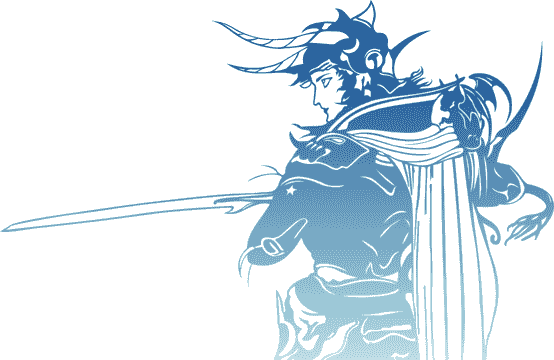
\includegraphics[width=\columnwidth]{./art/images/ff1.png} \end{center}
%
La potencia en combate puede mejorarse aún más utilizando el \hypertarget{equip}{equipo} adecuado. Mientras que las \textbf{armas }aumentan el daño infligido, la \textbf{armadura} protege contra el daño recibido. Los \textbf{accesorios} son objetos varios que pueden complementar el equipo de un personaje. Además, todas las partes del equipo pueden proporcionar mejoras a los atributos u otros efectos útiles. Cada personaje puede llevar un arma, una armadura y dos accesorios. Cualquier personaje puede usar cualquier accesorio, pero los personajes solo pueden equipar las armas y armaduras específicas según su oficio. Además, los personajes pueden utilizar \textbf{Objetos}, que proporcionan beneficios rápidos dentro y fuera de combate, aunque se consumen después de su uso. Todos los objetos y posesiones no equipadas se guardan en el \textbf{Inventario} de tu personaje.
%
\vspace{0.5cm}
%
\subsubsection*{Comercio}
El equipo y los objetos pueden ser recolectados de enemigos derrotados y cofres de tesoro. También se obtienen como recompensa por completar una tarea determinada. Pero a menudo el grupo tendrá que comprar o vender cosas específicas en tiendas y/o a comerciantes. El dinero que se utiliza para el comercio se llama \textbf{Gil} y generalmente son monedas. Puedes intentar comprar y vender casi cualquier cosa, siempre que alguien esté dispuesto a comerciar.
%
\vfill
%
\example{Comercio}{
Terra y su grupo visitan una casa de subastas para pujar por objetos raros. Hoy es su día de suerte: el objeto subastado es... ¡un \hyperlink{chocobo}{Chocobo} que habla! El grupo está impresionado por esta criatura talentosa y decide ofrecer todos sus ahorros (un total de 10000 Gil). Al principio parece que están superando a todo el mundo, pero en el último segundo, un padre afectuoso puja por 500000 Gil y adquiere el Chocobo como regalo para su hijo. Tal vez el grupo tenga mejor suerte (o más dinero) la próxima vez...
}
%
\pagebreak
%
\subsubsection*{Mejorar el Equipo}
Las armas y armaduras pueden mejorarse hasta alcanzar niveles más altos para que sean aún más potentes. Todo el equipo comienza en nivel 1 y mejorarlo cuesta como mínimo una cantidad determinada de Gil y lleva varias horas de trabajo. El DJ puede aplicar restricciones adicionales a las mejoras, como la obtención de materiales específicos o alguien con la pericia suficiente para realizar la tarea. Los personajes no jugadores también pueden mejorar su equipo y, en consecuencia, pueden encontrarse en el mundo objetos de nivel superior. Un arma o armadura mejorada mantiene sus efectos especiales, aumenta su potencia y puede cambiar su nombre o apariencia según lo decida quien realice la mejora. Existen reglas especiales para algunos tipos de equipo que se explican en las \textbf{notas} a continuación. Las siguientes tablas muestran los costos y efectos de la mejora de armas y armaduras a diferentes Niveles. \\
%
\vfill
%
\begin{tcolorbox}[colback=white,toptitle=0pt,colframe=accent,tabularx={c@{\hspace*{1.2cm}}c@{\hspace*{1.2cm}}l},sharp corners=south,
 title={\hspace*{\fill} \textbf{Mejoras de Armas} \hspace*{\fill}}]	
 \textbf{Nivel} & \textbf{Daño} & \textbf{Coste de mejora} \\ \hline
 1 & 1d & 1000 Gil \\ \hline
 2 & 2d & 2000 Gil \\ \hline
 3 & 3d & No se puede mejorar \\ \hline
\end{tcolorbox}
%
\vfill
%
\begin{tcolorbox}[colback=white,toptitle=0pt,colframe=accent,tabularx={c@{\hspace*{0.75cm}}c@{\hspace*{0.8cm}}l},sharp corners=south,
 title={\hspace*{\fill} \textbf{Mejoras de Armaduras} \hspace*{\fill}}]	
 \textbf{Nivel} & \textbf{DEF / RES} & \textbf{Coste de mejora} \\ \hline
 1 & Ver notas & 1000 Gil \\ \hline
 2 & +1 / +1 & 2000 Gil \\ \hline
 3 & +1 / +1 & No se puede mejorar \\ \hline
\end{tcolorbox}
%
\vfill
%
\subsubsection*{Equipo Legendario}
Aparte de armas y armaduras normales, existe una clase de equipo especial que puede o no existir en el mundo llamada \hyperlink{leq}{Equipo legendario}. Son armas y armaduras extraordinariamente potentes y de gran relevancia y, en consecuencia, encontrarlas exige un esfuerzo tremendo. El equipo legendario siempre es único y no puede ser mejorado ni puede llegarse a él mejorando otro objeto.
%
\vfill
%
\subsubsection*{Ejemplos}
A continuación se muestran algunos objetos y equipo típicos. Todas las armas tienen un alcance de 1u por defecto. Todas las armas y armaduras de nivel 1 tienen un valor predeterminado de 500 Gil, excepto el equipo que no tiene efectos únicos (p. ej., \hyperlink{mknife}{Espada de Mythril}), que solo vale la mitad. Las listas dadas no son exhaustivas y se alienta al DJ a que realice cambios y agregue más equipo. Normalmente, el grupo comienza el juego con un equipo básico (p. ej., \hyperlink{mknife}{Espada de Mythril}), objetos (p. ej., \hyperlink{item}{Poción}) y algo de Gil. En lugar de armadura, los personajes también pueden llevar ropa ordinaria que solo proporciona DEF +1 y no se puede mejorar.
%
\pagebreak
%
\eweapon{Arcos}{weapon.png} {
	\hline Arco \newline de Mithril & -- \\
	\hline Arco \newline Oscuro & Si realizas 3 \hyperlink{action}{Ataques} exitosos sobre un objetivo con esta arma, inflige \hyperlink{status}{Ceguera} por 3 turnos. \\ 
	\hline Arco \newline Élfico & Siempre que realices un \hyperlink{action}{Ataque} sobre un objetivo que tenga algún \hyperlink{status}{Estado Alterado}, añade 1d al daño total. \\  
	\hline Arco \newline Asesino & Si logras hacer \hyperlink{action}{Daño Crítico}, el objetivo pasa instantáneamente a estar \hyperlink{status}{KO}. \\ 
	\hline \multicolumn{2}{p{0.95\columnwidth}}{\textbf{Nota:} Los arcos tienen un alcance de 5u. Si realizas un \hyperlink{action}{Ataque} con un arco, no puedes moverte en ese mismo turno.} }
\vfill
\eweapon{\hypertarget{mknife}{Dagas}}{weapon.png}{
	\hline Cuchillo \newline de Mithril & --\\
   	\hline Daga \newline de Asesino & Si logras hacer \hyperlink{action}{Daño Crítico}, el objetivo pasa instantáneamente a estar \hyperlink{status}{KO}. \\ 
   	\hline Gladius & La DC de todas las tiradas relacionadas con robar se reduce en 1.\\ 
   	\hline Main \newline Gauche & Si hay algún aliado tuyo a 1u del objetivo, añade 1d al daño infligido por \hyperlink{action}{Ataques} con esta arma. \\ 
}
\vfill
\eweapon{Armas de Fuego}{weapon.png} {
	\hline Pistola \newline de Mithril & --  \\ 
	\hline Fomalhaut & El daño infligido por esta arma es del tipo \hyperlink{type}{Mágico}. \\ 
	\hline Metralleta & Cuando realices un \hyperlink{action}{Ataque}, también puedes causar 1d daño a otro enemigo que se encuentre a 1u del objetivo original. \\ 
	\hline Tiny Bee & Después de cada \hyperlink{action}{Ataque}, inmediatamente puedes moverte 1u.\\  
   	\hline \multicolumn{2}{p{0.95\columnwidth}}{\textbf{Nota:} Las pistolas tienen un alcance de 3u. El daño de las armas de fuego no aumenta directamente por la FUE. En su lugar, su daño aumenta 1d por cada 3 puntos de FUE del usuario.} }
\vfill
\eweapon{Puños}{weapon.png}{
	\hline Puños \newline de Mithril & -- \\
	\hline Garra \newline de Gato & La DC de evasión del objetivo aumenta en 1 punto cuando recibe un \hyperlink{action}{Ataque} de esta arma. \\ 
	\hline Puño \newline del Káiser & Si realizas 3 \hyperlink{action}{Ataques} exitosos sobre un objetivo con esta arma, inflige \hyperlink{status}{Inmóvil} por 3 turnos. \\ 
	\hline Colmillos de Tigre & Siempre que el objetivo de tus \hyperlink{action}{Ataques} saque 3 o menos en la tirada de evasión, haces \hyperlink{action}{Daño Crítico}. \\ 
}
\pagebreak
\eweapon{Lanzas}{weapon.png}{
	\hline Lanza \newline de Mithril & --  \\ 
	\hline Gae Bolg & Tienes \hyperlink{check}{Ventaja} en todas las tiradas de iniciativa. \\ 
	\hline Longinus & Si realizas 3 \hyperlink{action}{Ataques} exitosos sobre un objetivo con esta arma, inflige \hyperlink{status}{Veneno} por 3 turnos. \\ 
	\hline Tridente & Esta arma daña al objetivo original y a quien esté directamente detrás de él.\\
	\hline \multicolumn{2}{p{\columnwidth}}{\textbf{Nota:} Las lanzas tienen un alcance de 2u.} }
\vfill
\eweapon{Bastones}{weapon.png}{
	\hline Bastón \newline de Mithril & --  \\ 
	\hline Bastón \newline Elemental & Esta arma debe ser de un elemento específico (p. ej., \hyperlink{type}{Fuego}) y puede tener un nombre acorde (p. ej., "Bastón de Fuego"). Cuando causes daño de ese elemento, añade 1d al total.\\ 
	\hline Bastón \newline Sanador & Cuando cures PV con una habilidad, añade 1d al total. \\ 
	\hline Bastón \newline de Lilith & Puedes evadir los \hyperlink{action}{Ataques} aún cuando estás concentrándote. \\ 
	\hline Bastón \newline de Malboro & Cuando utilices \hyperlink{action}{Magia} que inflija algún \hyperlink{status}{Estado Alterado} negativo, la DC que debe superar el objetivo aumenta 1 punto.\\ 
	\hline Vara \newline Estrellada & Si tienes más de 0 PM, puedes consumir tus PM restantes para lanzar \hyperlink{action}{Magia} con un costo superior al valor que tienes disponible. \\ 
	\hline \multicolumn{2}{p{0.95\columnwidth}}{\textbf{Nota:} Los bastones aumentan un punto de MAG por nivel de arma (por ejemplo, un bastón de Nivel 1 da MAG~+1). A cambio, los bastones no aumentan su daño cuando se mejoran.} }
\vfill
\eweapon{\hypertarget{sword}{Espadas}}{weapon.png}{
	\hline Espada \newline de Mithril & -- \\ 
	\hline Espada Mortal & Cada vez que hagas \hyperlink{action}{Daño Crítico}, haces el cuádruple de daño (en vez del doble). \\ 
	\hline Sable-pistola & Siempre que utilices una habilidad, puedes hacer un \hyperlink{action}{Ataque} adicional a distancia con un alcance de 3u. Para este Ataque, no sumas tu FUE al daño.\\ %L6
	\hline Joyeuse & Siempre que inflijas un \hyperlink{status}{Estado Alterado}, aumenta 1 turno a su duración. \\
	\hline Organyx & Cuando hagas un \hyperlink{action}{Ataque} sobre un enemigo, recuperas 1d de PM. \\
	\hline Viva \newline la Reina & Cuando tú o un aliado a 1u de distancia sea dañado por \hyperlink{action}{Magia}, puedes reducir el daño a la mitad si pasas una DC de 9. \\ 
}
\pagebreak
\earmor{Armadura Pesada}{armor.png}
{
	\hline Armadura \newline Mithril & --  \\ 
	\hline Malla \newline de Cristal & Resiste: \hyperlink{type}{Hielo} \\
	\hline Malla\newline de Demonio & Resiste: \hyperlink{type}{Oscuro} \\ 
	\hline Armadura\newline de Diamante & Resiste: \hyperlink{type}{Eléctrico} \\ 
	\hline Malla \newline de Dragón & Resiste: \hyperlink{type}{Eléctrico} \\ 
	\hline Armadura\newline de Caballero & FUE +1 \\ 
	\hline Malla \newline de Espejo & Inmunidad: \hyperlink{status}{Silencio} \\
	\hline \multicolumn{2}{p{0.95\columnwidth}}{\textbf{Nota:} Toda armadura pesada proporciona DEF +2 en el nivel 1 de armadura.}
}
\vfill
\earmor{Armadura Ligera}{armor.png}
{
	\hline Chaleco \newline de Mithril & -- \\ 
	\hline Equipo de Gaia & Resiste: \hyperlink{type}{Tierra} \\
	\hline Traje Kenpogi & Inmunidad: \hyperlink{status}{Ceguera} \\ 
	\hline Minerva & Resiste: \hyperlink{type}{Hielo} \\
	\hline Chaleco de \newline Espejismo & Inmunidad: \hyperlink{status}{Sueño} \\ 
	\hline Equipo de Ninja & Inmunidad: \hyperlink{status}{Inmóvil} \\ 			 
	\hline Chaleco \newline de Poder & FUE +1 \\ 
	\hline Chaqueta Roja & Resiste: \hyperlink{type}{Fuego} \\ 
	\hline Chaleco de \newline Supervivencia & +5 a los PV máximos \\ 
	\hline \multicolumn{2}{p{0.95\columnwidth}}{\textbf{Nota:} Toda armadura ligera proporciona DEF +1 y RES +1 en el nivel 1 de armadura.} }
\vfill
\earmor{Túnicas}{armor.png}
{
	\hline Túnica \newline de Seda &  --  \\
	\hline Túnica \newline Negra & Inmunidad: \hyperlink{status}{Veneno} \\
	\hline Túnica de \newline Algodón & Resiste: \hyperlink{type}{Viento} \\ 
	\hline Túnica \newline Luminosa & Resiste: \hyperlink{type}{Sagrado} \\ 
	\hline Túnica \newline de Mago & MAG +1 \\ 
	\hline Túnica \newline de Erudito & +5 a los PM máximos \\
	\hline Túnica \newline Blanca & Inmunidad: \hyperlink{status}{Sueño} \\  
	\hline \multicolumn{2}{p{0.95\columnwidth}}{\textbf{Nota:} Todas las túnicas proporcionan RES +2 en el nivel 1 de armadura.} }
\pagebreak
\lweapon{\hypertarget{leq}{Armas Legendarias}}{weapon.png} {
	\hline Arma \newline Omega & Cualquiera & +10 a los PV máximos. \newline Esta arma puede ser de cualquier tipo (p. ej. Espada). \\ 
	\hline Arma \newline Artema & Cualquiera & +10 a los PM máximos. \newline Esta arma puede ser de cualquier tipo (p. ej. Espada). \\  
	\hline Artemisa & Arco & Los \hyperlink{action}{Ataques} que provengan de este arco no pueden ser esquivados. \\ 
	\hline Matamagos & Daga & Reduce los PM del objetivo en la misma cantidad que los PV de daño infligidos. \\ 	
	\hline Pena \newline de Muerte & Arma de \newline Fuego & Cuando inflijas el estado \hyperlink{status}{KO} a un enemigo, puedes hacer inmediatamente otro \hyperlink{action}{Ataque}.\\
	\hline Mano \newline de Dios & Puño & El daño infligido por esta arma es del tipo \hyperlink{type}{Mágico} y \hyperlink{type}{Sagrado}. \\  
	\hline Gungnir & Lanza & Cuando caes sobre un enemigo luego de un Salto, infliges 1d de daño \hyperlink{type}{Eléctrico}. \\
	\hline Nirvana & Bastón & Cuando lanzas \hyperlink{action}{Magia} que inflige daño o recupera PV, obtienes 1d adicional. \\
	\hline Maza \newline de Zeus & Bastón & Cuando lanzas \hyperlink{action}{Magia} con éxito, recuperas 1d de PM. \\    
	\hline Excalibur & Espada & Al atacar, añade 1d de daño \hyperlink{type}{Sagrado}. \\ 	
	\hline Masamune & Espada & Los daños provocados por esta arma ignoran \hyperlink{type}{Resistencia}. \\ 	
	\hline Ragnarok & Espada & Cuando tus PV están por debajo del 10 \% de su valor máximo, cada \hyperlink{action}{Ataque} exitoso contra un enemigo hace \hyperlink{action}{Daño Crítico} \\ 
	\hline \multicolumn{3}{p{0.95\columnwidth}}{\textbf{Nota:} Todas las armas legendarias infligen 4d de daño y están sujetas a las reglas específicas de su tipo.} }
\vfill
\lweapon{Armadura legendaria}{armor.png}{ 
	\hline Armadura Genji & Armadura Pesada & FUE +2 \\ 
	\hline Maximillian & Armadura Pesada & +10 a los PV máximos. \\ 
	\hline Atuendo \newline Negro & Armadura ligera & Tienes \hyperlink{check}{Ventaja} en todas las tiradas de iniciativa. \\ 
	\hline Traje \newline de Héroe & Armadura ligera & Todos los beneficios recibidos de \hyperlink{status}{aumATR} se duplican.\\ 	
	\hline Túnica de los Señores & Túnica & Resiste: \hyperlink{type}{Daño elemental} \\ 
	\hline Túnica \newline de Sabio & Túnica & +10 a los PM máximos \\ 
	\hline \multicolumn{3}{p{0.95\columnwidth}}{\textbf{Nota:} Todas las armaduras legendarias otorgan +4 a DEF y RES.} }

\accessory{Accessories}{acc.png}
{
	\hline Mythril Shield & 500 Gil & DEF +1  \\ 
    \hline Power Armlet & 500 Gil & STR +1 \\ 
    \hline Rune \newline Bracers & 500 Gil & RES +1 \\
   	\hline Battle Boots & 750 Gil & Immunity: \hyperlink{status}{Immobile}  \\
 	\hline Silver Glasses & 750 Gil & Immunity: \hyperlink{status}{Blind}  \\   
	\hline Star \newline Pendant & 750 Gil & Immunity: \hyperlink{status}{Poison}  \\
	\hline White Cape & 750 Gil & Immunity: \hyperlink{status}{Silence}  \\ 	
	\hline Thief Gloves & 1000 Gil & You have \hyperlink{check}{Advantage} on all checks related to \hyperlink{thief}{stealing}. \\ 
    \hline Protect Ring & 1250 Gil & Whenever you suffer an \hyperlink{action}{Attack}, you gain \hyperlink{status}{EnDEF} for 1 round.\\
    \hline Circlet & 1500 Gil & RES +1, MAG +1\\
    \hline Grand \newline Helmet & 1500 Gil & STR +1, DEF +1\\  
    \hline Safety Bit & 1500 Gil & Immunity: \hyperlink{status}{KO}  \\ 
    \hline Champion Belt & 2000 Gil & STR +1, \newline Immunity: \hyperlink{status}{DeATR} \\ 
    \hline Germinas Boots & 2500 Gil & You can jump twice as high as usual.  \\  
   	\hline Black Belt & 3000 Gil & Maximum HP +10  \\ 
   	\hline Moogle Charm & 4000 Gil & Glows when there is a monster within 50u of you.  \\  
    \hline Hero's Shield & 5000 Gil & DEF +1, RES +1, \newline Immunity: \hyperlink{status}{Sleep}\\
    \hline Feather Boots & 6000 Gil & You can levitate up to 1u above the ground. \\
    \hline Hermes Sandals & 7000 Gil & AGI~+1 \\
    \hline Genji \newline Helmet & 9000 Gil & Resilience: \hyperlink{type}{magical}\\  
    \hline Genji Shield & 9000 Gil & Resilience: \hyperlink{type}{physical}\\ 
   	\hline Genji Gloves & 9999 Gil & Whenever you make an \hyperlink{type}{Attack}, you can make a second one immediately after.  \\ 
   	\hline Ribbon & 9999 Gil & Immunity: \hyperlink{status}{All Status Effects}  \\
   	\hline Gold \newline Hairpin & 9999 Gil & Whenever you use \hyperlink{action}{Magic}, the MP cost is halved.  \\  
   	\hline Dragon Seal & ??? Gil & Proof of slaying a dragon god. \\
   	\hline Omega Badge & ??? Gil & Proof of defeating an ancient weapon. \\ 
	\hline \multicolumn{3}{p{0.95\columnwidth}}{\textbf{Note:} For some accessories it does not make sense to wear two of the same type (e.g. shields).}
}
\consumables{Items}{item2.png}
{
	\hline Gysahl Greens & 25 Gil & Vegetable well-known as a \hyperlink{chocobo}{Chocobo's} favorite food. \\
	\hline Antidote & 50 Gil & Removes \hyperlink{status}{Poison}.\\ 
	\hline Eyedrops & 50 Gil & Removes \hyperlink{status}{Blind}.  \\ 
	\hline Echo Grass & 50 Gil & Removes \hyperlink{status}{Silence}.  \\ 
	\hline Gold \newline Needle & 50 Gil & Remove \hyperlink{status}{Immobile}. \\ 
	\hline Arctic Wind & 100 Gil & The target suffers 2d \hyperlink{type}{ice} damage. \\
	\hline Bomb Fragment & 100 Gil & The target suffers 2d \hyperlink{type}{fire} damage.  \\
	\hline Lightning Gem & 100 Gil & The target suffers 2d \hyperlink{type}{lightning} damage. \\ 
	\hline Potion & 100 Gil & The target regains 2d HP.  \\ 
	\hline Holy\hspace{0.05cm}Water & 150 Gil & Removes \hyperlink{status}{Zombie}.  \\
	\hline Light \newline Curtain & 200 Gil & The target gains \hyperlink{status}{EnDEF} for 3 rounds. \\
	\hline Lunar \newline Curtain & 200 Gil & The target gains \hyperlink{status}{EnRES} for 3 rounds.  \\
	\hline Malboro Vine & 250 Gil & The target makes a DC 8 check and suffers \hyperlink{status}{Poison} for 3 rounds upon failure. \\
	\hline Remedy & 250 Gil & Removes all status effects, except \hyperlink{status}{KO}.  \\ 
	\hline Sleeping Powder & 250 Gil & The target makes a DC 8 check and suffers \hyperlink{status}{Sleep} for 3 rounds upon failure. \\
	\hline Ether & 300 Gil & The target regains 2d MP.\\ 	
	\hline Hero Drink & 300 Gil & The target gains \hyperlink{status}{EnSTR} and \hyperlink{status}{EnMAG} for 3 rounds. \\
	\hline Warp Stone & 300 Gil & You teleport to a place you can see within 10u. \\
	\hline Hi-Potion & 400 Gil & The target regains 6d HP.  \\ 
	\hline Phoenix Down & 500 Gil & Removes \hyperlink{status}{KO} and the target regains 1 HP.\\ 
	\hline Dark \newline Matter & 500 Gil & The target suffers 8d \hyperlink{type}{dark} damage \\
	\hline Turbo Ether & 750 Gil & The target regains 6d MP. \\
	\hline Mega-Potion & 800 Gil & Everyone within 1u regains 6d HP.  \\  
	\hline Elixir & 1000 Gil & The targets fully regains HP and MP. \\ 
	\hline Tent & 1000 Gil & Allows the party to sleep outside comfortably. \\
	\hline Gold \newline Hourglass & 1500 Gil & Time freezes for everyone except yourself within 5u for 20 seconds (2 rounds).  \\
	\hline Mega-Elixir & 2000 Gil & Everyone within 1u fully regains their HP and MP. \\
	\hline Mega-Phoenix & 3000 Gil & Removes \hyperlink{status}{KO} from everyone within 1u and fully recovers their HP and MP. \\
}
\pagebreak
\twocolumn

